%===================================== CHAP 2 =================================

\chapter{Background}


\section{Evolution}

In nature, evolution is the process governing change and preservation of
hereditary traits in populations of biological organisms. It allows species to
adapt to their environment over generations through reproduction, variation and
survival of the fittest \cite{Darwin1859}.

Artificial evolution seeks to harness the powerful adaptive capabilities of
natural evolution and apply them to general problem solving and learning. While
research on the subject has branched into many different sub-areas, the general
concept of optimizing a population of individuals with respect to some fitness
function using mechanisms inspired by natural evolution, is referred to using
the umbrella term Evolutionary Algorithm (EA) \cite{Holland1975}.

One of the greatest strengths of EAs is how universally applicable they are. EAs
have successfully been applied to many different problem domains, such as
robotics \cite{Floreano2000}, bioinformatics \cite{KosakovskyPond2006},
medicine \cite{Fitzgerald:2015:IAS:2739480.2754761} and many more.

\subsection{Goldberg, GA}

The most common type of EA is perhaps the Genetic Algorithm (GA) \cite{Goldberg:1989:GAS:534133}.

\begin{figure}[ht]
  \centering
  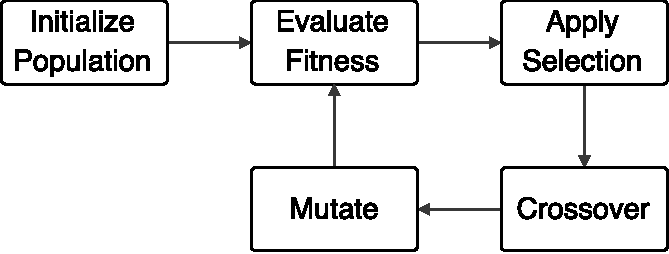
\includegraphics[width=0.5\linewidth]{fig/ga}
  \caption{Genetic Algorithm process.}
  \label{fig:ga}
\end{figure}



\subsection{Koza, Genetic programming}

Genetic Programming (GP) is an area of research in artificial evolution aiming
to program computers through evolution. Programs represented as tree structures
are encoded as genotypes and evolved subject to some fitness function using a
GA. By mutating genotypes through operations that preserve the 

\section{Development}

Biological development is the natural process that allows complex multi-cellular
organisms to be built starting from a single cell using instructions encoded in
the DNA of the organism. The most easily recognizable example is the development
of humans from a single cell, the zygote, containing the combined genetic
material of the parents, through cell division and differentiation. The human
genome does not contain an exhaustive description and blueprint of each
individual human. Rather, it consists of instructions governing how cells should
divide and differentiate based on their surrounding cells and feedback from the
environment.

Developmental processes in nature have many properties that make them desireable
to mimic through artificial development. For instance, the number of cells in
the human body is orders of magnitudes larger than the amount of information
encoded in our DNA \cite{Bianconi2013}. In general, the performance of GAs and
GP implementations decline as the size of the genome increases, as mutations are
more likely to be detrimental with regards to fitness. By introducing
development as an indirect mapping between genotype and phenotype, programs and
structures that scale to arbitrary dimensions can be produced while still
maintaining a search space that the EA method in question can efficiently
explore. Systems that combine evolution and development in this way are often
referred to as EvoDevo systems \cite{Hall2003}.

Where evolution allows a species to adapt over the span of generations,
development continues throughout the lifetime of each individual, allowing for
adaption based on changes to the environment. This makes EvoDevo particularily
well suited in the design of robust and environment-insensitive artificial
intelligence agents.

\section{Cellular Computation}

Embryogenesis evolved to develop 3D structures from linear code, not to create
Universal Turing Machines

\subsection{Developmental Cellular Architectures}

\tikzstyle{block} = [draw, fill=white!20, rectangle, 
    minimum height=2em, minimum width=5em]
\tikzstyle{sum} = [draw, fill=blue!20, circle, node distance=1cm]
\tikzstyle{input} = [coordinate]
\tikzstyle{output} = [coordinate]
\tikzstyle{pinstyle} = [pin edge={to-,thin,black}]
\begin{figure}[ht]
  \begin{adjustbox}{max size={\textwidth}}
  \begin{tikzpicture}
  [help lines/.style={draw=black},
  every node/.style={help lines,rectangle,minimum size=3mm},
  cellular automaton/.style={draw=none,row sep=0mm,column sep=0mm, ampersand replacement=\&, label=above:#1},
  cellular automaton2/.style={draw=none,row sep=0mm,column sep=0mm, ampersand replacement=\&, label=below:#1},
  w/.style={fill=white,help lines},
  b/.style={fill=black, help lines},
  r/.style={fill=red, help lines},
  g/.style={fill=black!30!green,help lines}]

    \matrix (DS0) [cellular automaton={DS 0}] {
      \node[w] {};\& \node[w] {};\& \node[w] {};\& \node[w] {};\& \node[w] {}; \\
      \node[w] {};\& \node[w] {};\& \node[w] {};\& \node[w] {};\& \node[w] {}; \\
      \node[w] {};\& \node[w] {};\& \node[g] {};\& \node[w] {};\& \node[w] {}; \\
      \node[w] {};\& \node[w] {};\& \node[w] {};\& \node[w] {};\& \node[w] {}; \\
      \node[w] {};\& \node[w] {};\& \node[w] {};\& \node[w] {};\& \node[w] {}; \\
    };
    \matrix (DS1) [cellular automaton={DS 1}, right=of DS0] {
      \node[w] {};\& \node[w] {};\& \node[w] {};\& \node[w] {};\& \node[w] {}; \\
      \node[w] {};\& \node[w] {};\& \node[g] {};\& \node[w] {};\& \node[w] {}; \\
      \node[w] {};\& \node[g] {};\& \node[g] {};\& \node[g] {};\& \node[w] {}; \\
      \node[w] {};\& \node[w] {};\& \node[r] {};\& \node[w] {};\& \node[w] {}; \\
      \node[w] {};\& \node[w] {};\& \node[w] {};\& \node[w] {};\& \node[w] {}; \\
    };
    \matrix (SS0) [cellular automaton2={SS 0}, below left=of DS1] {
      \node[w] {};\& \node[b] {};\& \node[w] {};\& \node[w] {};\& \node[b] {}; \\
      \node[b] {};\& \node[w] {};\& \node[w] {};\& \node[w] {};\& \node[w] {}; \\
      \node[w] {};\& \node[w] {};\& \node[b] {};\& \node[b] {};\& \node[w] {}; \\
      \node[w] {};\& \node[b] {};\& \node[w] {};\& \node[w] {};\& \node[w] {}; \\
      \node[w] {};\& \node[b] {};\& \node[b] {};\& \node[w] {};\& \node[b] {}; \\
    };
    \matrix (SS1) [cellular automaton2={SS 1}, right=of SS0] {
      \node[w] {};\& \node[b] {};\& \node[w] {};\& \node[w] {};\& \node[b] {}; \\
      \node[b] {};\& \node[w] {};\& \node[b] {};\& \node[w] {};\& \node[w] {}; \\
      \node[w] {};\& \node[b] {};\& \node[w] {};\& \node[b] {};\& \node[w] {}; \\
      \node[w] {};\& \node[b] {};\& \node[w] {};\& \node[w] {};\& \node[w] {}; \\
      \node[w] {};\& \node[b] {};\& \node[b] {};\& \node[w] {};\& \node[b] {}; \\
    };
    \matrix (SSN) [cellular automaton2={SS N}, right=of SS1] {
      \node[w] {};\& \node[b] {};\& \node[w] {};\& \node[w] {};\& \node[b] {}; \\
      \node[b] {};\& \node[w] {};\& \node[w] {};\& \node[w] {};\& \node[w] {}; \\
      \node[w] {};\& \node[w] {};\& \node[b] {};\& \node[w] {};\& \node[w] {}; \\
      \node[w] {};\& \node[b] {};\& \node[w] {};\& \node[w] {};\& \node[w] {}; \\
      \node[w] {};\& \node[b] {};\& \node[b] {};\& \node[w] {};\& \node[b] {}; \\
    };
    \matrix (SS01) [cellular automaton2={SS 0}, right=of SSN] {
      \node[w] {};\& \node[b] {};\& \node[w] {};\& \node[w] {};\& \node[b] {}; \\
      \node[b] {};\& \node[w] {};\& \node[w] {};\& \node[w] {};\& \node[w] {}; \\
      \node[w] {};\& \node[w] {};\& \node[b] {};\& \node[w] {};\& \node[w] {}; \\
      \node[w] {};\& \node[b] {};\& \node[w] {};\& \node[w] {};\& \node[w] {}; \\
      \node[w] {};\& \node[b] {};\& \node[b] {};\& \node[w] {};\& \node[b] {}; \\
    };
    \matrix (SS11) [cellular automaton2={SS 1}, right=of SS01] {
      \node[w] {};\& \node[b] {};\& \node[b] {};\& \node[w] {};\& \node[b] {}; \\
      \node[b] {};\& \node[w] {};\& \node[b] {};\& \node[w] {};\& \node[w] {}; \\
      \node[b] {};\& \node[b] {};\& \node[w] {};\& \node[b] {};\& \node[w] {}; \\
      \node[w] {};\& \node[b] {};\& \node[w] {};\& \node[w] {};\& \node[w] {}; \\
      \node[w] {};\& \node[b] {};\& \node[w] {};\& \node[w] {};\& \node[b] {}; \\
    };
    \matrix (SSN1) [cellular automaton2={SS N}, right=of SS11] {
      \node[w] {};\& \node[b] {};\& \node[w] {};\& \node[w] {};\& \node[b] {}; \\
      \node[b] {};\& \node[w] {};\& \node[b] {};\& \node[w] {};\& \node[w] {}; \\
      \node[w] {};\& \node[w] {};\& \node[w] {};\& \node[w] {};\& \node[b] {}; \\
      \node[w] {};\& \node[b] {};\& \node[b] {};\& \node[w] {};\& \node[w] {}; \\
      \node[w] {};\& \node[b] {};\& \node[b] {};\& \node[w] {};\& \node[b] {}; \\
    };
    \matrix (DS2) [cellular automaton={DS 2}, above=of SS11] {
      \node[w] {};\& \node[w] {};\& \node[g] {};\& \node[w] {};\& \node[w] {}; \\
      \node[w] {};\& \node[w] {};\& \node[g] {};\& \node[w] {};\& \node[w] {}; \\
      \node[g] {};\& \node[g] {};\& \node[g] {};\& \node[g] {};\& \node[g] {}; \\
      \node[w] {};\& \node[w] {};\& \node[r] {};\& \node[w] {};\& \node[w] {}; \\
      \node[w] {};\& \node[w] {};\& \node[g] {};\& \node[w] {};\& \node[w] {}; \\
    };

    \node[draw=none] at ($(SS1)!.5!(SSN)$) {\ldots};
    \node[draw=none] at ($(SS11)!.5!(SSN1)$) {\ldots};

    \draw[->] (DS0) -- (DS1);
    \draw[->] (DS1) -- (DS2);
    \draw[->] (SS0) -- (SS1);
    \draw[->] (SS01) -- (SS11);
    \draw[black] (DS1.south west) -- (SS0.north west);
    \draw[black] (DS1.south east) -- (SSN.north east);
    \draw[black] (DS2.south west) -- (SS01.north west);
    \draw[black] (DS2.south east) -- (SSN1.north east);
    \draw[thick, ->] (2, 2) -- (12,2) node[midway, above, draw=none] {Time};
  \end{tikzpicture}
  \end{adjustbox}
  \caption{
    Development starting from a single green cell using the growth
    rule in Figure~\ref{fig:growth-rules}.
  }\label{fig:dev-example}
\end{figure}

\begin{figure}[ht]
  \centering
  \begin{tikzpicture}[g/.style={draw, minimum size=3mm,   
        fill=black!30!green},w/.style={draw, minimum size=3mm},r/.style={draw, minimum size=3mm, fill=red},
      m/.style={matrix of nodes, column sep=1pt, row sep=1pt, draw, label=below:#1}, node distance=1pt]

    \matrix (A) [m={Gw}]{
      &|[w]|\\
      |[w]|&|[w]|&|[g]|\\
      &|[w]|\\
    };
    \matrix (B) [m={Gn}, right=of A]{
      &|[w]|\\
      |[w]|&|[w]|&|[w]|\\
      &|[g]|\\
    };
    \matrix (C) [m={Ge}, right=of B]{
      &|[w]|\\
      |[g]|&|[w]|&|[w]|\\
      &|[w]|\\
    };
    \matrix (D) [m={Gs1}, right=of C]{
      &|[g]|\\
      |[w]|&|[r]|&|[w]|\\
      &|[w]|\\
    };
    \matrix (E) [m={Gs2}, right=of D]{
      &|[r]|\\
      |[w]|&|[g]|&|[w]|\\
      &|[w]|\\
    };
  \end{tikzpicture}
  \caption{
    Growth rules for a cellular developmental system where cells are
    either empty or of the green type.
  }\label{fig:growth-rules}

\end{figure}
\clearpage

\section{Reservoir Computing}

\subsection{Spiking Neural Networks as Readout Layers}

\todo{Rewrite}

Artificial neural networks can be grouped into three generations, based on the characteristics of their base computational unit, the neuron.
The first generation, based on McCulloch-Pitts neurons~\cite{McCulloch1943}, simple threshold gates, allows for universal computation on digital input/output values.
In the second generation, neurons apply a non-linear, continuous activation function on the weighted sum of their inputs.

The third generation of networks bases itself on spiking neurons, which model the interaction between biological neurons more closely.
In this model, a neuron $v$ fires when its potential $P_v$ exceeds a threshold $\theta_v$.
The potential is, at any time, the sum of the postsynaptic potentials, resulting from firing of presynaptic neurons.
The contribution of a spike from presynaptic neuron $u$ at time $s$ to the potential $P_v$ of postsynaptic neuron $v$ is given by $w_{u,v} \cdot \varepsilon_{u,v}(t-s)$, where $w_{u,v}$ is a weight representing the strength of the synapse connecting $u$ and $v$, and $\epsilon_{u,v}(t-s)$ models the response of the spike as a function of time passed since the spike occurred.
A synapse can be both excitatory and inhibitory, meaning that its contribution to the total potential $P_v$ can be both positive and negative.
A biologically plausible response function is shown in figure~\ref{fig:response-function-snn}.
From a machine learning perspective, the trainable part of a spiking neural network, is the weight $w_{u,v}$, determining to what degree spikes from a neuron $u$ influences the potential of neuron $v$.

In~\cite{Maass1997}, Maass shows that spiking neurons are at least computationally equal to the models used in generation one and two, and that they can also be more efficient in terms of neurons required to compute a function.
SNNs also have the required attributes to be used as a reservoir in an RC system~\cite{Pipa2010}.
In order to be able to create an efficient implementation of a RC-machine based on a cellular developmental system as described in~\ref{sec:rc-machine}, being able to perform classification in the spiking domain is essential.

\section{Related Work}
\cleardoublepage
%%% Local Variables:
%%% mode: latex
%%% TeX-master: "../thesis"
%%% End:
